\chapter{Crittografia}
L'idea iniziale della crittografia era quella di creare una comunicazione privata all'interno di 
un ambiente pubblico, dove un terzo individuo potrebbe essere in ascolto di
una comunicazione in atto tra le due parti. La crittografia moderna è basata
su sofisticati formalismi matematici, che però rendono possibile una sua
applicazione in un contesto pratico. Al giorno d'oggi non è richiesto saper
progettare nuovi sistemi crittografici, ma saper utilizzare quelli odierni,
dei quali è già stata dimostrata la validità. Oggi giorno è quindi utilizzata
tra due controparti della comunicazione, per scambiarsi un messaggio in codice
(\textbf{crittogramma}) all'interno di un canale non ritenuto sufficientemente
sicuro (all'interno del canale può esistere un intruso, detto \textbf{crittoanalista},
che è in ascolto delle comunicazioni che avvengono all'interno del canale): il 
mittente codificherà il messaggio in chiaro (\textit{plaintext}) in uno
cifrato (\textit{ciphertext}) tramite una funzione di codifica $C: m\to c$: questo
verrà quindi intercettato dal destinatario che lo convertirà tramite una funzione
di decodifica $D: c\to m$. 

In particolare, queste due funzioni in questione necessiteranno di una chiave
per effettuare la codifica o la decodifica: possiamo quindi esprimere le due
funzioni (che matematicamente sono inverse) come:
\[C_k(m)=c\quad D_k(c)=m\quad D_k(C_k(m))=m\]
In più, se si ha che $C_k(D_k(m))=D_k(C_k(m))=m$, allora si dice che le due 
funzioni sono \textit{commutative}, in quanto l'ordine con il quale esse vengono
applicate con le loro rispettive chiavi è irrilevante. In particolare, in questa
situazione, l'intruso non dovrà essere a conoscenza della funzione di decodifica
D.

Tuttavia dobbiamo anche possedere un'infrastruttura atta a mantenere 
il sistema crittografico; possiamo avere sicurezza tramite crittografia in due
modi:
\begin{description}
\item[Segretezza perfetta] questa implica che una parte dell'informazione 
	necessaria alla decodifica non dovrà mai essere divulgata; è per tanto
	facilmente intuibile che questa è impossibile da ottenere
\item[Segretezza computazionale] questa implica una disparità di risorse tra
	l'avversario ed il suo antagonista; queste sono ovviamente le risorse
	di calcolo, che dovranno essere supposte limitate superiormente (al
	di sopra delle quali non si garantisce la confidenzialità).
\end{description}
Sappiamo inoltre che i nostri messaggi saranno di dimensione finita ($N$)
e che essa è trasmessa nella rete tramite bit, che vogliamo trasmettere in
un modo confidenziale. Un ascoltatore potrebbe modificare gli $N$ bit per vedere,
con una probabilità di $\frac{1}{2^N}$, se riceve una risposta esatta: abbiamo
conseguentemente che esso avrà una probabilità molto bassa di ottenere un 
risultato corretto, anche con un $N$ modesto. 


Diciamo quindi che un algoritmo di crittografia è ottimale se un ascoltatore
non può fare meglio di $\frac{1}{2^N}$ per poter decifrare il nostro crittogramma,
con la quale possiamo perseguire una forma debole di segretezza perfetta.
Diamo ora le seguenti definizioni:
\begin{description}
\item[Crittografia] consiste nella progettazione di cifrari sicuri ed efficienti
\item[Crittoanalisi] consta nell'insieme dei metodi, degli strumenti
	e delle tecniche per attaccare i cifrari,  eventualmente per
	testarne la loro qualità, ma per lo più per intenti malevoli. Questo
	lavoro è svolto dal \textbf{crittoanalista}.
\item[Crittologia] è l'insieme di crittografia e crittoanalisi
\end{description}

In particolare il sistema di crittografia si chiama \textbf{simmetrico} o a \textbf{chiave
privata} se l'origine
e la destinazione utilizzano una stessa chiave $k$ per le funzioni di coding
e decoding, spesso con $C\equiv D$; se invece le due chiavi non coincidono
il sistema di crittografia si dice \textbf{asimmetrico} o a \textbf{chiave pubblica}.

Possiamo inoltre distinguere due differenti famiglie di algoritmi crittografici,
in base alla segretezza delle funzioni di codifica e di decodifica:
\begin{description}
\item[Cifrari per uso ristretto] C e D sono mantenute segrete; questi cifrari
	possono quindi essere utilizzati solamente quando non si vuole tenere
	un elevato grado di sicurezza, e quando si è all'interno di un contesto
	molto semplificato (si ha appunto sicurezza tramite non divulgazione).
\item[Cifrari per uso generale] C e D sono note a tutti, e quindi la segretezza
	della comunicazione si basa sulla segretezza della chiave.
\end{description}

Tuttavia non è solo con la crittografia che possiamo mantenere la confidenzialità
dei nostri dati; bisogna mantenere:
\begin{description}
\item[Integrità] il destinatario deve controllare che il messaggio ricevuto 
	non abbia subito delle modifiche parziali o totali durante il tragitto
\item[Autenticazione] il destinatario deve poter accertare che il messaggio
	provenga esattamente da un destinatario noto, ovvero vogliamo la 
	garanzia che il messaggio sia giunto da un preciso mittente.
\item[Non-repudiation] in quanto è garantita l'autenticazione, il mittente
	non può disconoscere il messaggio da lui inviato: se ciò è dimostrabile,
	il messaggio può essere conservato come prova dell'effettivo mittente
\end{description}

\section{Metodi d'attacco}
L'intruso, all'interno della comunicazione, può avere sia un ruolo \textit{passivo}
(ovvero, ascolta solamente la comunicazione come all'interno delle intercettazioni
telefoniche; questa forma risulta naturale all'interno delle reti wireless), 
oppure \textit{attivo} (non solo è in ascolto della comunicazione, ma
interviene all'interno di questa andando ad introdurre propri bit, od andando
a modificare direttamente quelli dell'utente; questa forma risulta semplice
nella modalità Man-In-The-Middle). 

Un intruso può effettuare in questo contesto tre tipologie d'attacco:
\begin{description}
\item[Cyphertext attack] si salvano tutti i crittogrammi che fluiscono all'interno
	della rete, sui quali poi si effettuerà la crittoanalisi; da questi
	poi si tenterà di ottenere il plaintext.
\item[Known plain-text attack] partendo dal presupposto che si conosca il 
	plain-text di alcuni crittogrammi, l'intruso prova ad ottenere il 
	plain-text anche degli altri che trova all'interno della rete.
\item[Chosen plain-text attack] si presuppone che il crittoanalista abbia a
	disposizione una serie di messaggi in chiaro, che può criptare ottenendo
	i corrispondenti crittogrammi.
\end{description}

\section{Crittografia simmetrica o a chiave privata}
D'ora in poi, nelle sezioni seguenti, partiremo dal presupposto di conoscere
le funzioni $C$ e $D$; con questo metodo di crittografia, è come se chiudessimo
all'interno di uno scrigno l'informazione che, sia la destinazione sia il mittente
sono in grado di carpire, tramite una chiave che entrambi conoscono (e 
conseguentemente anche il lucchetto per accedere all'informazione sarà sempre
riconosciuto da entrambi).

In questo scenario tuttavia lo scambio della chiave deve avvenire \textbf{out of
band}, ovvero al di fuori del canale di comunicazione che si crede non sicuro,
in quanto un potenziale intruso potrebbe carpire la chiave ed utilizzare per
decifrare i messaggi che verranno trasportati da una parte all'altra,
compromettendo conseguentemente l'utilizzo della chiave stessa nella comunicazione
criptata. Possiamo quindi trasportare la chiave all'interno di un'intranet,
tramite un mezzo personale o tramite telefono, etc. Comunque il canale secondario per la distribuzione della chiave, deve
essere scelto in un modo proporzionale al valore del messaggio trasmesso, che
deve costituire un canale meno rintracciabile rispetto a quello dove avverrà 
la normale comunicazione. Analogamente, la stessa chiave non potrà essere
utilizzata all'infinito, in quanto dopo un certo periodo di tempo è da considerarsi
compromesso, in quanto sarà aumentata la probabilità che un malintenzionato
sia riuscito ad ottenerla; tuttavia bisogna sottolineare che la segretezza della
chiave dipenderà dal mantenimento della segretezza da entrambe le contro parti.
 Inoltre, queste chiavi dovranno avere una lunghezza
considerevole, in modo che risulti sconveniente effettuare un attacco brute force
per ottenerla, e dovranno essere \textit{confidenziali} in quanto, non potendo
distinguere a priori gli amici dai nemici, non sappiamo se quello che utilizzerà
la nostra chiave sarà interessato ad intercettare le nostre comunicazioni. Alcuni 
cifrari simmetrici sono \textit{DES}, \textit{triple DES}, \textit{AES}
ed \textit{IDEA}.

Possiamo inoltre notare che, per ogni $n$ utenti, si avrà necessità di possedere
$n^2$ chiavi simmetriche, e saranno necessari 
$\frac{n(n-1)}{2}$ canali per scambiarsi la comunicazione\footnote{Si divide per
due perché dobbiamo considerare il nostro canale di comunicazione bidirezionale}.


\section{Crittografia asimmetrica o a chiave pubblica}
Vogliamo ora capire se è possibile mantenere la confidenzialità senza effettuare 
lo scambio di una chiave segrete tra le controparti della comunicazione. Questa
risoluzione è infatti di interesse economico, in quanto elimina la parte di 
comunicazione out of band, che è un grosso handicap per il sistema simmetrico.


In questo particolare sistema è il desitnatario che sceglie un ``lucchetto'' ed
un'apposita chiave, fornendo unicamente il primo (aperto) al mittente: questo
si preoccuperà di chiudere l'informazione con tale lucchetto, e di spedire
lo scrigno così ottenuto a destinazione, la quale potrà aprire il suo lucchetto
tramite la chiave che essa stessa ha generato. In questo modo può avvenire una
qualsiasi forma di comunicazione tra A e B, senza che questi si conoscano
precedentemente; nota inoltre che, se l'ordine di consegna dei lucchetti e delle
chiavi fosse invertito, non sarebbe possibile alcuna forma di comunicazione
privata.


Questi algoritmi devono inoltre garantire che sia difficile desumere la funzione di codifica
da quella di decodifica, sempre non conoscendo al chiave privata (che si traduce quindi in un attacco di tipo
brute force per desumerne il valore); questo concetto si applica per 
transizione anche alle funzioni di codifica e decodifica, implicando sempre la
non conoscenza della chiave privata: si parla infatti di funzione \textbf{one-way trap-dor}:
\begin{enumerate}
\item Si dice che è ``a senso unico'' in quanto se la funzione C
	è semplice da conoscere, deve essere complicato ottenere la funzione 
	inversa D
\item Si dice che è una ``botola'' in quanto se non conosco la chiave giusta,
	non devo essere in grado di rompere il meccanismo
\end{enumerate}
Un esempio di applicazione di queste formule è direttamente correlato alla
teoria dei numeri primi: dati due numeri primi $p$ e $q$ infatti sufficientemente
grandi (ovvero con centinaia di cifre), è facile calcolare $n=pq$, ma è difficile
ottenere uno dei due numeri primi dato $n$ (sappiamo che la fattorizzazione
degli stessi è infatti un problema arduo, in quanto l'algoritmo che risolverebbe
questo problema è appunto superpolinomiale), sempre supposto di non conoscere
l'altro. Conseguentemente abbiamo che possiamo ottenere la chiave pubblica dal
numero $n$ così ottenuto, che avrà alpiù il doppio di cifre dei numeri primi
dati in partenza.


Con questo scenario, sarà sufficiente distribuire a tutti gli utente una sola 
chiave (quella pubblica), e ogni destinatario potrà generare una propria chiave
privata per tutte le comunicazioni future.

\section{Cifrari storici}
\subsection{Cifrari a sostituzione}
Il \textbf{cifrario di Cesare} è basato sul principio di \textit{sostituzione} dei caratteri
tramite traslazione verso destra o sinistra di $k$ posizioni dell'alfabeto
criptato rispetto a quello originale (\textit{shift ciclico}); in questo cifrario
avremo inoltre una chiave costituito da un solo numero, che viene utilizzato
per ogni lettera:
\[C(m_i)=(pos(m_i)+k)\mod 26=c_i\quad D(c_i)=(pos(m_i)-k)\mod 26\]
Analogamente, potremo generalizzare questo cifrario imponendo una qualsiasi
sostituzione del nostro carattere con un altro; in questo modo passiamo da
26 possibili chiavi a un numero di $26!-1$ trasformazioni, in quanto ogni 
trasformazione è una permutazione dell'alfabeto. Tuttavia, entrambi questi
cifrari possono essere soggetti all'attacco di tipo statistico: l'ascoltatore
occulto infatti potrebbe confrontare il campione statistico di una lingua nota
con quelli desunti da un campione di crittogrammi, ed assegnare la lettera
in plain-text che in quella lingua occorre con la maggior frequenza con quella
che occorre più frequentemente nei crittogrammi; se questa formulazione dovesse
rivelarsi errata, si potrà procedere per confronto con tutte le altre lettere.
Altri cifrari a sostituzione implicano:
\begin{itemize}
\item Si ottiene una chiave di lunghezza $|k|$, che viene replicata per tutta
	la lunghezza del messaggio: si effettua poi una sostituzione del carattere
	del messaggio $m_i$ con quella della chiave $k_j$ prendendo il 
	carattere $T[m_i,k_j]$ all'interno di una tabella.
\item Si può effettuare la sostituzione tra blocchi di caratteri: 
\end{itemize}

\subsection{Cifrari a Trasposizione}
Si stabilisce una chiave che stabilisce una chiave con numeri unici e 
distinguibili, che identificano una permutazione arbitraria della disposizione
del messaggio. Si dispone poi il messaggio per righe facendolo coincidere con
la lunghezza della chiave; in seguito si leggono le colonne ottenute dal messaggio
in base all'ordine fornito dalla chiave.

In questi cifrari non andrà più a buon fine l'attacco di tipo statistico, in
quanto la frequenza di occorrenza delle lettere sarà identica a quella del
messaggio originale, ma sarà cambiata unicamente la disposizione delle lettere.

Si può inoltre ripetere la tecnica dettagliata precedentemente, finchè non 
otterrò un output ancora più sicuro in quanto in questo
	modo aumento l'entropia (ad ogni combinazione è sempre meno evidente che il crittogramma
	possa essere ottenuto tramite riordinamneto, sembrando quindi un messaggio casuale), poiché riordiniamo i caratteri in
	un modo ancora più casuale del precedente.

Nota: con una scelta inappropriata della chiave si potrebbe rischiare di 
ottenere esattamente lo stesso messaggio di partenza, anche se effettivamente
questo non è lo scopo del nostro algoritmo. Si può inoltre notare che, mentre
con una sola trasposizione si riscontrano regolarità nell'andamento delle 
posizioni del messaggio, via via che le trasposizioni successive aumentano
l'ordine di decodifica diventa sempre meno chiaro.

\subsection{Cifrario One-Time Pad}
Questo cifrario è anche detto cifrario perfetto, in quanto è un caso limite che 
esplica quale elevato grado di codifica possiamo ottenere con le tecniche di
crittografia.

Dato un messaggio di lunghezza $|n|$, possiamo ottenere una chiave casuale (per 
questo il cifrario è detto \textbf{one-time}, anche perché viene utilizzata
una sola volta per spedire un solo messaggio) della
stessa lunghezza detta \textbf{pad}: possiamo ottenere il crittogramma effettuando
lo xor bit a bit tra messaggio e pad. Possiamo inoltre notare che, dato il 
crittogramma e la chiave, possiamo di nuovo ottenere il messaggio originale
effettuando sempre lo xor bit a bit. 

Ora passiamo a trattare la sicurezza dell'algoritmo: abbiamo che la nostra
chiave è generata casualmente (ottenuta con probabilità $\frac{1}{2^n}$), ed 
abbiamo che anche l'intruso avrà tale probabilità di ottenere la chiave: infatti,
sapendo che viene utilizzato l'operatore XOR, se l'$i$-esimo bit della chiave è
0, allora il bit del testo cifrato sarà lo stesso del messaggio, altrimenti questo dovrà essere invertito:
per questo si dice che è un ``cifrario perfetto''.

Tuttavia abbiamo immediatamente che questo algoritmo non è applicabile in
pratica in quanto risulta molto costoso: infatti in quanto la chiave è unica
per ogni nuovo invio del messaggio, il costo dell'invio della chiave privata
tramite un altro canale di comunicazione sicuro non verrà mai ammortizzato; 
inoltre si ha sempre un costo per lo scambio della chiave proporzionale alla 
lunghezza del messaggio stesso.

\subsection{DES}
\begin{figure}[!t]
 \centering
   \subfloat[][\emph{Trattazione generale dell'algoritmo}.]{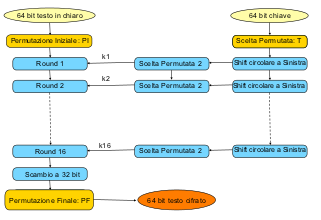
\includegraphics[scale=0.75]{images/des_up.png}}
   \subfloat[][\emph{Analisi del punto $k_i$ di 16}.]{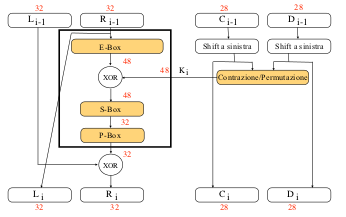
\includegraphics[scale=0.75]{images/des_under.png}}
 \caption{\emph{DES Overview}}\label{fig:des}
\end{figure}
Prima di introdurre questo cifrario, descriviamo alcune tecniche che possono
essere utilizzate all'interno degli algoritmi di cifrazione:
\begin{description}
\item[Permutazione] cambiamento dell'ordine del messaggio
\item[Sostituzione] indico a quale blocco ne corrisponderà un altro nel messaggio
	cifrato
\item[Espansione] replicazione all'interno di un messaggio di un bit o di un 
	carattere
\item[Contrazione] (detta anche scelta), 
	alcuni caratteri o bit vengono scartati e poi permutati: quando 
	successivamente si effettua una permutazione, allora l'insieme di 
	queste due operazioni viene detta \textbf{scelta permutata}.
\end{description}
Come si può vedere dall'immagine \vref{fig:des} \emph{(b)}, la chiave (rappresentata
da $C_k$ e $D_k$) è costituita da due blocchi formanti complessivamente 56 
bit, contro i due blocchi da 32 bit (complessivamente 64) del messaggio: questo
perché i rimanenti 8 bit della chiave sono di parità. Dobbiamo inoltre evidenziare
che \texttt{E-Box} indica un'espansione, \texttt{S-Box} una sostituzione e \texttt{P-Box}
una permutazione.

\subsection{RSA}
Questo è un algoritmo di crittografia a chiave pubblica, del quale recentemente
è scaduto il brevetto. Esso sfrutta la teoria dei numeri e la definizione
della funzione di Eulero\footnote{La funzione di Eulero è quella che associa
ad ogni naturale $n$ il numero dei naturali $m$ primi con $n$ tali che $m\leq n$,
ed è indicato come $\varphi(n),n\neq 1$. Si può dimostrare che:
\begin{itemize}
\diam Se $n$ è primo allora $\varphi(n)=n-1$ (tutti i numeri primi con lui
	saranno tutti quelli minori di lui, tranne il numero stesso)
\diam Se $n$ è una potenza di un primo, allora $\varphi(n^r)=n^r-n^{r-1}$, ovvero
	a tutti i numeri fino ad $n^r$ tolgo tutti quei numeri che sono multipli
	di $n$ fino ad $n^r$, che sono appunto $n^{r-1}$.
\diam Se $a$ e $b$ sono coprimi, allora $\varphi(ab)=\varphi(a)\varphi(b)$
\diam Segue che per un qualsiasi numero $n$ scomponibile per la fattorizzazione
	standard (che si dimostra essere unica) nel modo $n=\prod^i a_i^{e_i}$
	con $a_i$ primo, è scrivibile come $\varphi(n)=n\prod^i\left(1-\frac{1}{a_i}\right)$
\end{itemize}
}: dati due numeri primi $p$ e $q$, si dimostra che $\varphi(pq)=(p-1)(q-1)$.
Diciamo inoltre che, i numeri primi che sceglieremo, non dovranno essere 
contemplati da nessuna fonte facilmente reperibile, in quanto sarebbe immediato
decifrare la chiave pubblica per ottenere quella privata. In particolare
dobbiamo trovare:
\[\exists e. GCD(e,\varphi(n))=1\quad \exists d.d\cdot e\,\textrm{mod}\varphi(n)=1\]
dove costituiranno le chiavi:
\[\textrm{pubblica} = (e,n)\quad\textrm{privata} = (d,n)\]
Da questo si può quindi ricavare la formula per effettuare la codifica del 
messaggio:
\[C(m)=m^e\text{ mod }n = c\]
In questa funzione, dato il messaggio che si vuole cifrare $m$, l'utente 
conosce mediante la sua chiave privata i valori di $e$ ed $n$. Inoltre è 
possibile elevare a potenza $e$ un messaggio, considerandolo come costituito
da bit, e conseguentemente come un numero. La funzione di decodifica risulta
quindi la seguente:
\[D(c)=c^d\text{ mod } n = m\]
Il destinatario è inoltre in grado di effettuare questo calcolo in quanto 
conosce i valori di $d$ ed $n$ tramite la sua chiave pubblica. 

Giunti a questo punto, non abbiamo tuttavia dimostrato nè la correttezza, né la
sicurezza e nemmeno l'efficienza del calcolo di questo algoritmo, in quanto i 
calcoli da svolgere possono essere considerevoli. Ci appresteremo
or ora nella loro trattazione.

\subsubsection{Correttezza}
Per dimostrare la correttezza dell'algoritmo, dobbiamo provare che le due funzioni
di codifica e decodifica siano inverse, ovvero che $D(C(m))=m$. Prima di 
effettuare la dimostrazione, dobbiamo prendere in considerazione i seguenti
risultati:
\begin{itemize}
\diam $GCD(m,n)=1\;\Rightarrow\; m^{\Phi(n)}\text{ mod }n=1$ (Teorema di Eulero)
\diam $m^k\text{ mod }p=1\wedge m^k\text{mod }q=1\;\Rightarrow\; m^k\text{ mod }pq=1$
\diam $x\text{ mod }n=1\;\Rightarrow\; \forall y. x^y\text{ mod }n=1$
\end{itemize}
Possiamo inoltre supporrre che $m$ sia un messaggio tale che $0<m<n$: tuttavia,
non sempre potremo avere la garanzia che tale messaggio sia della dimensione
desiderata; in questo caso potremo operare come in DES, ovvero dividendo il 
messaggio in ingresso in parti .
\begin{proof}
Applicando il valore delle funzioni in $D(C(m))$, otterremo:
\[\begin{split}
D(C(m))&=D(m^e\text{ mod }n)\\
       &=(m^e\text{ mod }n)^d\text{ mod }n\\
       &= m^{ed}\text{ mod }n
\end{split}\]
In quanto abbiamo per definizione dell'argoritmo e quindi per imposizione che
$de\text{ mod }\Phi(n)=1$, quindi abbiamo che $\exists k>0. de = k\Phi(n)+1$.
Possiamo quindi riscrivere l'esponente dell'espressione di cui sopra come segue,
utilizzando anche il teorema di Eulero:
\[\begin{split} 
D(C(m)&=\dots\\
      &=mm^{k\Phi(n)}\text{ mod }n=m\cdot 1=m
\end{split}\]
\end{proof}
\subsubsection{Sicurezza}
In quanto sappiamo che l'unica nostra arma di sicurezza è quella di generare
chiavi lunghe ($N\to\infty$) in modo tale che $\frac{1}{2^N}\to0$, ovvero
di generarle casualmente tramite un attacco di forza bruta, proviamo ad 
evidenziare due possibili metodi di attacco:
\begin{itemize}
\item Riuscire a fattorizzare $n$ in modo da ottenere i valori di $p$ e $q$ primi
      che si sanno esistenti
\item Dal valore di $n$ ottengo $\Phi(n)$, ed in seguito riesco ad ottenere
      $d=e^{-1}\text{ mod } \Phi(n)$, grazie ai dati che conosco dalla chiave
      pubblica
\end{itemize}
Possiamo quindi riscontrare che entrambi questi metodi hanno una complessità che
è pari al costo di fattorizzare $n$, in quanto per ottenere $\Phi(n)$ devo saper
fattorizzare $n$. Tuttavia fin'ora non è ancora stato trovato un risultato
teorico che dimostri il costo computazionale del lower-bound di questo problema,
e sono state portate unicamente delle evidenze empiriche sulla difficoltà
strutturale nella risoluzione del problema: ci si affida unicamente al fatto che
sia improbabile che qualcuno entro breve scopra il valore di suddetto lower-bound.

Come abbiamo potuto constatare dalle osservazioni precedenti, la sicurezza degli
algoritmi di crittografia fa affidamento sulle esigue risorse a disposizione
degli attaccanti: per questo, con l'evolversi della tecnologia, si trova sempre
più necessario trovare dei valori di numeri primi sempre più grandi. Altra
garanzia di sicurezza è dovuta al fatto che, riuscire a decomporre un numero $n$
in due numeri primi, non implica essere in grado di effettuare la fattorizzazzione
di $n'\neq n$ in un minor tempo, sempre considerando che $n'$ non è composto
dagli stessi fattori primi di $n$. 

\subsubsection{Efficienza}
Ora vogliamo trovare delle tecniche per rendere più efficienti i calcoli del nostro
algoritmo:
\begin{description}
\item[Esponenziale] per computare $n^{32}$, invece di effettuare 31 operazioni di 
		    moltiplicazione, potremo operare nel modo seguente:
		    \[x^{2y}=x^y\cdot x^y\quad x^{y+1}=xx^y\]
		    In questo modo possiamo semplificare i conti se consideriamo
		    l'esponente in binario: considerando le cifre da sinistra
		    verso destra, eleveremo il risultato precedente al quadrato
		    se il bit successivo è zero (sarebbe moltiplicare per due),
		    altrimenti moltiplichiamo un'altra volta per $x$. In questo
		    caso, detto $y$ l'esponente, nel caso pessimo effettueremo
		    sempre $2\log_2 y$ moltiplicazioni
\item[Modulo] in quanto i nostri calcoli sono sempre sotto modulo $n$, allora 
		    possiamo verificare che:
		    \[(a\text{ mod }n)(b\text{ mod }n)\text{ mod } n = (ab)\text{ mod }n\]
		    In questo modo, invece di effettuare sempre il calcolo del
		    modulo alla fine, lo possiamo effettuare per ogni passo
		    intermedio, in modo da evitare l'overflow, in quanto appunto
		    il risultato finale che otterremo non potrà mai essere più
		    grande di $n$.
\end{description}

\subsubsection{Test di primalità}
Sempre correlato alla sicurezza dell'algoritmo, parliamo ora dei test di 
primalità che possono essere ricondotti alla sicurezza dell'algoritmo. Come
prima cosa, abbiamo una probabilità di $\frac{1}{\ln(n)}$ che un dato numero
primo $n$ sia primo. Tuttavia questa probabilità, sebbene sia molto bassa, non
è zero, e quindi l'evento può sempre avvenire.

Possiamo quindi effettuare dei test di primalità, che rispondono se un numero
è primo o meno. In un metodo Naïf potremo scandire tutti gli interi da $2$ a
$n-1$, ma un risultato teorico ci consente di limitare ulteriormente questo
numero con $\sqrt n$. Detto quindi $m=\log n$ la dimensione del nostro numero
in input, otteniamo complessivamente una complessità $O(\sqrt n)=O(2^{\frac{1}{2}n})$.
Non si sono trovati inoltre, se non recentemente, dei risultati polinomial per
il test di primalità: utilizzando l'\textit{Ipotesi di Riemann} si arriva ad un
$O((\log n)^4)$, mentre con l'algoritmo AKS si arriva ad un $O((\log n)^6)$:
tuttavia, anche se il risultato è polinomiale, abbiamo che è lo stesso un
risultato inefficiente, in quanto la costante è considerevolmente elevata.

Abbiamo inoltre il seguente risultato dal \textit{Teorema di Fermat}\footnote{Come
conseguenza del teorema di eulero}:
\[\mathtt{prime}(n),0<a<n\Rightarrow a^{n-1}\text{ mod }n=1\]
\textit{Pomerance} ha inoltre ottenuto la probabilità che venga superato il test
$a^{n-1}\text{ mod }n=1$ da un numero non primo con $\forall. a<n$, che è $\frac{1}{10^{13}}$.
Possiamo quindi generare un algoritmo del tipo:
\begin{pseudoc}
int isprime(int *n) {
  *n = random_dispari();
  a = random() % *n;
  return  ((a**(*n-1) % *n)==1);
}
\end{pseudoc}
Tuttavia, se il test è passato, è ancora presente $\frac{1}{10^{13}}$ di probabilità
che il numero non sia primo: in questo modo possiamo ripetere il nostro test di cui
sopra per tanti $a$ generati casualmente, in quanto testo il mio numero $n$ per
$k$ volte,  in questo modo avrò effettuato prove del test per tanti valori di
$a$, abbassando ulteriormente ad un $\frac{1}{10^{{13}^k}}$ la probabilità di
fallimento del test. Si testeranno quindi $\frac{\log(n)}{2}$ numeri prima di
accettare il numero come primo.

\section{Identificazione, autentiticazione e firma digitale}
In quanto ci possiamo accorgere che con la sola crittografia non possiamo aver
garantita la confidenzialità, sono state introdotte le segueti funzionalità:
\begin{description}
\item[Identificazione] dobbiamo essere in grado di accertare l'identità di un
	utente che vuole accedere ai suoi servizi
\item[Autentificazione] vogliamo accertare che il messaggio ricevuto sia di un
	predefinito utente, e che il messaggio ricevuto sia giunto integro
\item[Firma digitale] vogliamo accertarci che un documento sia stato scritto
	da un prefissato mittente (da utilizzare quando non c'è reciproca fiducia
	tra le due estremita della comunicazione).
\end{description} 

\subsection{Funzioni di Hash}
Per introdurre i concetti di firma dei messaggi che seguiranno, è importante 
definire che cosa siano le funzioni di Hash. Dato un dominio $X$ contentente le
\textit{pre-image}, ovvero i valori che dovranno essere mappati nel codominio
$Y$ degli hash-value; tale valore risultante è chiamato \textbf{digest} o
\textbf{fingerprint}.  Il nostro requisito è che, data una funzione $f:X\to Y$, 
del tipo ``many-to-one'', ovvero $|X|>|Y|$ di molti ordini di grandezza.

Questa sarebbe una proprietà propria di ogni funzione di hasing. Tuttavia nel
campo della crittografia e della sicurezza richiediamo delle altre caratteristiche:
\begin{itemize}
\diam Visto che la funzione è del tipo ``many-to-one'', vogliamo che i nostri
	valori siano distribuiti all'interno di un'area uniforme.
	Dato un sottoinsieme del dominio degli elementi che hanno tutti la stessa
	immagine, ovvero $X_i=\Set{x\in X|f(x)=y_i}$, vogliamo che questi sottodomini
	siano distribuiti in una maniera uniforme, ovvero che:
	\[\forall X_i.\exists c. |X_i|\simeq c\]
\diam Inoltre vogliamo che elementi $\forall x_i\in \mathbb I(x)$ appartengano
	a sottoinsiemi distinti e ben distanziati, ovvero:
	\[\forall x_i,x_j\in\mathbb I(x).x_i\in X_a\wedge x_j\in X_b,\; a\ll b \vee b\ll a\] 
	Questa dispersione all'interno delle hash table garantisce che non 
	avrò mai la collisione per valori molto vicini all'interno della tabella,
	in modo da non rendere lenta la ricerca.
\diam Altre proprietà invece garantiscono che le funzioni di crittografia definite
	siano definibili come ``one-way'':
	\begin{itemize}
	\item $\forall x\in X. f(x)$ deve essere facilmente computabile
	\item $\forall y\in Y. \exists x. f(x)=y$ deve essere arduo da calcolare
	\item $\forall x_1\in X. \exists x_2\in X. f(x_1)=f(x_2)$ deve essere arduo da calcolare
	\end{itemize}
\end{itemize}

Proviamo a dare un semplice (fin troppo) algoritmo di funzione di hash, detta
\textit{simple 8-bit block parity}: dato un qualunque messaggio $m$, disponiamo il
messaggio su righe parallele previa suddivisione in blocchi da 8 bit, colmando
con un padding di zero l'ultimo blocco nel caso in cui avesse una dimensione inferiore
a quella prefissata. Il numero di digest si effettua calcolando il bit di parità
per quella colonna, ovvero effettuando lo XOR tra ogni bit. Da ciò segue naturalmente
che il fingerprint sarà sempre di una dimensione di 8 bit, con una possibilità
di $2^8$ valori possibili (è quindi il valore di $|Y|$), mentre $|X|$ è arbitraria.
Si può tuttavia dimostrare facilmente che questo non soddisfa le ultime due proprietà
dell'ultimo punto di cui sopra:
\begin{itemize}
\item in quanto il bit di parità mi fornisce un'informazione sul valore precedente
	di quel bit, posso ridurre la casistica dei valori possibili che seguono
	dimezzandola
\item è conseguentemente facile ottenere un messaggio della stessa partità
\end{itemize}

\subsection{Firma digitale}
Introduciamo ora la questione della firma digitale, facendo un parallelo
con quella manuale:
\begin{description}
\item[Authentic] Deve essere generabile solamente da una data persona, e quindi
	deve essere unica (un esempio è la calligrafia di chi scrive la firma).
\item[Unforgeable] Non deve essere facilmente falsificabile: non
	possiamo quindi utilizzare una firma come una stringa di bit da apporre
	in un documento, poiché altrimenti sarebbe evidente il plagio. (Nel mondo
	reale si distinguerebbe dalla calligrafia)
\item[Not Reusable] Segue che non deve essere riutilizzabile per altri
	documenti, impedendone sostanzialmente la copiabilità
\item[Unalterable] Una volta che il documento è stato firmato, non deve essere
	possibile cambiare il contenuto del documento.
\item[Non repudiation] Segue inoltre che, garantendo con la firma che l'utente
	mittente esiste, esso non potrà mai, una volta riconosciuto il documento
	come integro, ripudiarne il contenuto.
\end{description}

In quanto possiamo garantire con alcune funzioni la loro commutatività,
possiamo definire delle funzioni in questo modo:

\[A:s=D(m,k_A[priv])\Rightarrow \Braket{A,m,s}\quad\quad B:\mathtt{cmp}(C(s,k_A[pub]),m)\]

In questo modo avremo che il mittente firmerà il messaggio con la sua chiave privata
che lo identifica precisamente (e quindi non può ripudiare il documento non manipolato),
 è inoltre possibile applicare $D$ ad un qualsiasi 
valore numerico in virtù della proprietà di cui sopra, mentre conoscendo
$A$ il destinatario potrà conoscere la chiave pubblica del nostro mittente, che 
è disponibile a chiunque in modo gratuito.
Inoltre, in questo modo, la firma non è riutilizzabile, poichè strettamente 
legata al documento che è stato firmato, che quindi non risulta modificabile
a patto di minare l'integrità della codifica. 
Tuttavia con questa tecnica avremo un messaggio spedito dell'ordine di grandezza
di $2|m|$, ed il messaggio non risulta confidenziale poiché ognuno lo potrebbe
decodificare.\footnote{In quanto il messaggio è presente in chiaro, e perché
l'altro è ottenibile in lettura tramite la chiave pubblica.}

Per ovviare a questo fatto viene utilizzato un secondo modello:

\[A:s=D(m,k_A[priv])\wedge c=C(s,k_B[pub])\Rightarrow\Braket{A,c}\quad\quad B:m=C((\mathbf{s=D(c,k_B[priv])}),k_A[pub])\]

In questo caso non sono in grado di controllare se il messaggio è stato
inviato correttamente oppure no, se non tramite la correttezza del messaggio
dal punto di vista linguistico. A questo punto abbiamo che, se il messaggio è
una sequenza generica di bit, non possiamo in alcun modo controllare l'integrità
del messaggio o meno.

Segue che possiamo utilizzare un terzo protocollo, dove utilizziamo anche il
digest cifrato del nostro messaggio (per effettuare un controllo sul messaggio)
nel modo seguente.

\[A:s=D(f_h(m),k_A[priv])\wedge c=C(m,k_B[pub])\Rightarrow \Braket{A,c,s} \quad\quad B:f(D(c,k_B[priv]))==C(s,k_A[pub])\]

In questo modo autentico il messaggio con la mia chiave pubblica, ma firmo il 
digest tramite una chiave privata che manitene tutte e cinque le proprietà di una
firma.

\subsection{Autentificazione}
Per quanto concerne il \textit{Reply Attack}, dobbiamo inoltre considerare la validità 
di un messaggi in base
al tempo che si impiega tra invio e ricezione dello stesso. Il problema è che
un man in the middle, potrebbe ricevere il messaggio ed inoltrare ripetutamente
il messaggio alla destinazione: si rende quindi necessario applicare al messaggio
un \textit{time stamp} che possa indicare la scadenza. 

Ora, per stabilire l'identità di un utente, abbiamo che il messaggio deve
essere riconosciuto come fattura di un determinato utente, e conseguentemente
deve essere riconosciuta l'integrità del nostro messaggio.


Tramite una chiave segreta, condivisa da mittente e destinatario, si può
ottenere un'immagine di dimensione costante rispetto alla potenziale lunghezza
del messaggio, che può essere utilizzata per autenticare il messaggio, senza 
tuttavia possedere la proprietà di \textbf{non-repudiation}.

In questo caso possiamo utilizzare quindi un MAC (\textit{Message Authenticatin Code}),
tramite un messaggio breve e di lunghezza fissata, ottenibile tramite una chiave
segreta condivisa tra mittente e destinatario.

Dopo aver definito come $mk$ la concatenazione tra messaggio e chiave segreta 
alla fine dello stesso (che tuttavia entrambi conoscono), possiamo ottenere

\[A:\Braket{\mu=C_k(m),\omega=f_h(mk)}\quad\quad \mathtt{cmp}(\omega,f_k(D_k(\mu)k)); \] 


Abbiamo quindi identificazione poiché l'intruso non conosce $k$, ed aggiungendo
il fatto che $f_h()$ è one-way, ammettiamo anche confidenzialità, ed in quanto
non può modificare $m$, preserviamo l'integrità.
